% !TEX root = ../axiomatic.tex

\begin{notation}
	For $U \in \P_{n-i}^n$ we write $u \notin U$ if $u \in \{0, \dots, n\} \setminus U$. If $u \notin U$ define $u.U = \{u\} \union U \in \P_{n-i+1}(n)$ and if $u \in U$ define $U \setminus u = U \setminus \{u\} \in \P_{n-i-1}(n)$.
\end{notation}

\begin{notation}
	Given $\xi \colon \P_{n-i}(n) \to \F$ we denote by $\bar{\xi}$ the function with the same domain and range satisfying $\xi(U) \neq \bar{\xi}(U)$ for every $U$, and simplify the notation $U^{\xi(U)}$ and $U^{\bar{\xi}(U)}$ to $U^\xi$ and $U^{\bar{\xi}}$ respectively.
\end{notation}

\begin{lemma} \label{l:first nail}
	Let $\triangle$ be a free and non-degenerate cup-$i$ construction and $i,n \in \N$ with $i \leq n-2$.
	If there is a function $\xi \colon \P_{n-i}^n \to \F$ with
	\begin{equation} \label{e:assumed identity with xi and barxi}
	\triangle_i [n] \ = \!
	\sum_{U \in \P_{n-i}^n \kern-5pt} U^{\xi} \ot U^{\barxi}
	\end{equation}
	and either
	\[
	\triangle_i [n-1] = \Delta_i [n-1]
	\quad \text{or} \quad
	\triangle_i [n-1] = T\Delta_i [n-1],
	\]
	then $\xi$ is constant, i.e.,
	\[
	\triangle_i [n] = \Delta_i [n]
	\quad \text{or} \quad
	\triangle_i [n] = T \Delta_i [n].
	\]
\end{lemma}

\begin{proof}
	Let us assume $\triangle_i [n-1] = \Delta_i [n-1]$.
	The other case is proven analogously.
	Applying the boundary of $\cP(\simplex^n) \ot \cP(\simplex^n)$, as defined in \cref{e:boundary of P(simplex)}, to \cref{e:assumed identity with xi and barxi}	we have
	\begin{align*}
	\bd \, \triangle_i [n]\ & =\!
	\sum_{U \in \P_{n-i}^n \kern-5pt} \left(\sum_{u \notin U} {u.U^\xi} \ot {U^\barxi} \, +
	\sum_{u \notin U} {U^\xi} \ot {u.U^\barxi} \right) \\ & +\!
	\sum_{U \in \P_{n-i}^n \kern-5pt} \left(\sum_{u \in U^\barxi} {u.U^\xi} \ot {U^\barxi} \ +
	\sum_{u \in U^{\xi}} {U^\xi} \ot {u.U^\barxi} \right).
	\end{align*}
	By assumption and \cref{l:from the other paper} we have
	\[
	\triangle_i \bd \, [n] =
	\Delta_i \bd \, [n] \, = \!
	\sum_{U \in \P_{n-i}^n \kern-5pt} \left( \,
	\sum_{u \in U^1} {u.U^0} \ot {U^1} \, +
	\sum_{u \in U^0} {U^0} \ot {u.U^1} \right).
	\]
	Adding this last two identities together we have
	\begin{align}
	(1+T) \triangle_{i-1} [n] &= \bd \triangle_i [n] + \triangle_i \bd \, [n] \\ &=
	\label{e:top} \sum_{U \in \P_{n-i}^n \kern-5pt} \left(
	\sum_{\,u \notin U} u.U^\xi \ot U^\barxi \, +
	\sum_{u \notin U} U^\xi \ot u.U^\barxi \right) \\ &+ \,
	\label{e:bottom} (1+T) \sum_{\substack{U \in \P_{n-i}^n \\ \xi(U) \neq 0} \kern-3pt} \left(
	\sum_{\,u \in U^1} {u.U^0} \ot {U^1} \ +
	\sum_{u \in U^0} {U^0} \ot {u.U^1} \right).
	\end{align}
	We will use Lemma \ref{l:condition to be in the kernel of sxs} to show that summand \eqref{e:top} is in the kernel $K^{(j)}$ of $\cP(\sigma_j) \ot \cP(\sigma_j)$ for every codegeneracy $\sigma_j \colon [n] \to [n-1]$.
	Consider $U \in \P_{n-i}^n$.
	If $\{j, j+1\} \cap U = \emptyset$ then $u.U^\xi \ot U^\barxi \in K^{(j)}$ and $U^\xi \ot u.U^\barxi \in K^{(j)}$ for every $u \notin U$.
	If $\{j, j+1\} \cap U = \{j, j+1\}$ then the same conclusion follows from the fact that $\ind_U(j) = \ind_U(j+1)$.
	If $\{j, j+1\} \cap U = \{j\}$ then $u.U^\xi \ot U^\barxi \in K^{(j)}$ and $U^\xi \ot u.U^\barxi \in K^{(j)}$ for every $u \notin U$ with $u \neq j+1$.
	Furthermore, if $j \in U^\xi$ then $(j+1).U^\xi \ot U^\barxi \in K^{(j)}$ and $U^\xi \ot (j+1).U^\barxi \notin K^{(j)}$.
	An analogous statement holds if $j \in U^\barxi$ and a similar analysis applies to the case $\{j, j+1\} \cap U = \{j+1\}$.
	We will show that the basis elements in \eqref{e:top} that are not in $K^{(j)}$ cancel in pairs after the application of $\cP(\sigma_j) \ot \cP(\sigma_j)$.
	Let $\Gamma_j^\xi \subseteq \P_{n-i}^n$ consists of elements $U$ with $\{j, j+1\} \cap U = \{j\}$ and $j \in U^\xi$.
	Let $\Gamma_{j+1}^\xi$, $\Gamma_j^\barxi$, and $\Gamma_{j+1}^\barxi$ be defined analogously.
	The claim follows from the existence of the bijections $\Gamma_{j}^\xi \cong \Gamma_{j+1}^\xi$ and $\Gamma_{j}^\barxi \cong \Gamma_{j+1}^\barxi$ defined by the assignments $U \mapsto (j+1).\big( U \setminus \{j\} \big)$ and $U \mapsto j.\big( U \setminus \{j+1\} \big)$, since two summands related by one of these bijections are sent to the same element by $\cP(\sigma_j) \ot \cP(\sigma_j)$.

	We will impose conditions on summand \eqref{e:bottom} following an analysis similar to the one just given.
	Notice that $(1+T)$ commutes with $\cP(\sigma_j) \ot \cP(\sigma_j)$ and that the only basis elements in \eqref{e:bottom} not in $K^{(j)}$ are associated to pairs $(U, u)$ with $\xi(U) \neq 0$ and $u = j$ or $ u = j+1$.
	Let $\Lambda_{j}^0$ be the subset of $\{U \in \P_{n-i}^n \mid \xi(U) \neq 0\}$ consisting of sets $U$ with $j \in U^0$ and $j+1 \notin U$.
	We define $\Lambda_{j}^1$, $\Lambda_{j+1}^0$, and $\Lambda_{j+1}^1$ analogously.
	The set $\Lambda_{j \wedge j+1}$ is defined by the conditions $\xi(U) \neq 0$ and $j,j+1 \in U$.

	Observe that the sum
	\[
	\sum_{\Lambda_{j \wedge j+1}} \left( \sum_{u \in U^1} {u.U^0} \ot {U^1} +
	\sum_{u \in U^0} {U^0} \ot {u.U^1} \right)
	\]
	is in $K^{(j)}$ since, given that $\ind_U(j) = \ind_U(j+1)$, the only non-zero summands associated to $(U,j)$ and $(U,j+1)$ cancel each other.
	Therefore, applying $\cP(\sigma_j) \ot \cP(\sigma_j)$ to
	\[
	\sum_{\substack{\P_{n-i}^n \\ \xi(U) \neq 0}} \left(\sum_{u \in U^1} {u.U^0} \ot {U^1} +
	\sum_{u \in U^0} {U^0} \ot {u.U^1} \right)
	\]
	yields
	\begin{align*}
	&\sum_{\Lambda_{j}^0} U^0 \setminus \{j\} \ot {U^1} \ + \
	\sum_{\Lambda_{j}^1} U^0 \ot {U^1} \setminus \{j\} \\ + \
	&\sum_{\Lambda_{j+1}^0} U^0 \setminus \{j+1\} \ot {U^1} \ + \
	\sum_{\Lambda_{j+1}^1} U^0 \ot {U^1} \setminus \{j+1\}.
	\end{align*}
	which must be in the kernel of $(1+T)$.
	This implies the existence of an involution $\phi^{(j)}$ of $\Lambda = \Lambda^0_{j} \sqcup \Lambda^1_{j} \sqcup \Lambda^1_{j+1} \sqcup \Lambda^1_{j+1}$ defined by a choice of canceling pairs.
	By the freeness of $\Delta$ and since $i \leq n-2$, this involution has no fixed points.
	It follows that two elements $U$ and $U^\prime$ with $U \cap \{j, j+1\} = U^\prime \cap \{j, j+1\}$ cannot be related by $\phi^{(j)}$ since then $U = U^\prime$.
	Therefore, $\phi^{(j)}(U) = U^\prime$ if and only if $U^\prime = j.(U \setminus \{j+1\})$ or $U^\prime = (j+1).\big( U \setminus \{j+1\} \big)$.
	Recall that by definition $\xi(U) = \xi(U^\prime) \neq 0$.
	This analysis applies to any $j \in \{0, \dots, n\}$ and we introduce a relation in $\P_{n-i}^n$ writing $U \sim U^\prime$ if $U^\prime = j.(U \setminus \{j+1\})$ or $U^\prime = (j+1).\big( U \setminus \{j+1\} \big)$ for some $j$.
	By the previous analysis, if $U \sim U^\prime$ then $\xi(U) = \xi(U^\prime)$.
	The lemma now follows from observing that any two elements $V$ and $W$ in $\P_{n-i}^n$ are related by a sequence
	\[
	V \sim \dots \sim W,
	\]
	so $\xi \colon \P_{n-i}^n \to \F$ must be constant.
\end{proof}


\begin{lemma} \label{l:second nail}
	Let $\triangle$ be a free, non-degenerate and irreducible cup-$i$ construction and $i,n \in \N$ with $i \leq n-2$.
	If $\triangle_i [n] = \Delta_i [n]$ or $\triangle_i [n] = T \Delta_i [n]$ then the following implications hold:
	\begin{alignat*}{2}
	&\boxed{\triangle_i [n-1] = \Delta_i [n-1] \hspace*{7pt}}\ &\Longrightarrow\
	&\boxed{\triangle_i [n] = \Delta_i [n] \hspace*{7pt}} \\
	&\boxed{\triangle_i [n-1] = T \Delta_i [n-1]}\ &\Longrightarrow\
	&\boxed{\triangle_i [n] = T \Delta_i [n]} \ .
	\end{alignat*}
\end{lemma}

\begin{proof}
	We will establish the first of these implications using a proof by contradiction for which we assume $\triangle_i [n-1] = \Delta_i [n-1]$ and $\triangle_i [n] = T \Delta_i [n]$.
	The second implication is proven analogously.
	We have
	\begin{align*}
	(1+T) \triangle_{i-1}[n] &=
	\bd \triangle_i [n] + \triangle_i \bd \, [n] \\ &=
	\bd T \Delta_i [n] + \Delta_i \bd \, [n] \\ &=
	T \bd \Delta_i [n] + \bd \Delta_i [n] + \bd \Delta_i [n] + \Delta_i \bd \, [n] \\ &=
	(1+T) \bd \Delta_i [n] + (1+T) \Delta_{i-1} [n] \\ &=
	(1+T) \Delta_i \bd \, [n] + (1+T) \Delta_{i-1} [n].
	\end{align*}
	Using from \cref{l:from the other paper} that
	\[
	\Delta_i \bd \, [n] =
	\sum_{U \in \P_{n-i}^n \kern-5pt} \left( \,
	\sum_{u \in U^1} {u.U^0} \ot {U^1} \ +
	\sum_{u \in U^0} {U^0} \ot {u.U^1} \right)
	\]
	and that
	\[
	\Delta_{i-1} [n] \defeq
	\sum_{V \in \P_{n-i+1}^n \kern-15pt} V^0 \ot V^1
	\]
	we have
	\begin{align*}
	(1+T) \triangle_{i-1}[n] &=
	(1+T) \sum_{U \in \P_{n-i}^n \kern-5pt} \left( \,
	\sum_{u \in U^1} {u.U^0} \ot {U^1} \ +
	\sum_{u \in U^0} {U^0} \ot {u.U^1} \right) \\ &+
	(1+T) \sum_{V \in \P_{n-i+1}^n \kern-15pt} V^0 \ot V^1.
	\end{align*}
	By \cref{l:splitting of summands} there are functions $\eta \colon \P_{n-i}^n \to \F$ and $\zeta \colon \P_{n-i+1}^n \to \F$ such that
	\begin{align*}
	\triangle_{i-1}[n] \ &=
	\sum_{U \in \P_{n-i}^n \kern-5pt} \left( \,
	\sum_{u \in U^\bareta} u.U^\eta \ot U^\bareta \ +
	\sum_{u \in U^\eta} U^\eta \ot u.U^\bareta \right) \\ &+
	\sum_{V \in \P_{n-i+1}^n \kern-15pt} V^\zeta \ot V^\barzeta.
	\end{align*}
	But this contradicts the irreducibility of $\triangle$ as expressed in \cref{l:irreducubility recasted}.
\end{proof}


\begin{figure}
	\centering
	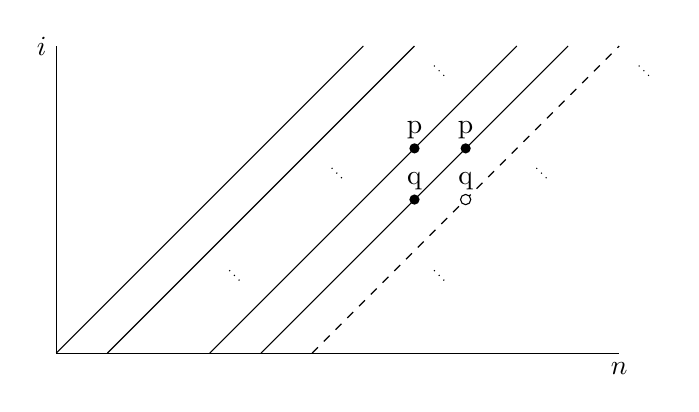
\begin{tikzpicture}[scale = .65]
	\draw (0,0)--(0,6);
	\draw (0,0)--(11,0);
	\draw (0,0)--(6,6);
	\draw (1,0)--(7,6);
	\draw (3,0)--(9,6);
	\draw (4,0)--(10,6);
	\draw[dashed] (5,0)--(11,6);

	\draw[dotted, shorten >=10pt,shorten <=10pt] (3,2)--(4,1);
	\draw[dotted, shorten >=10pt,shorten <=10pt] (5,4)--(6,3);
	\draw[dotted, shorten >=10pt,shorten <=10pt] (7,6)--(8,5);

	\fill (7,4) circle (0.1);
	\fill (8,4) circle (0.1);
	\fill (7,3) circle (0.1);
	\fill[white] (8,3) circle (0.1);
	\draw (8,3) circle (0.1);

	\node[above] at (7,4) {p};
	\node[above] at (8,4) {p};
	\node[above] at (7,3) {q};
	\node[above] at (8,3) {q};

	\draw[dotted, shorten >=10pt,shorten <=10pt] (7,2)--(8,1);
	\draw[dotted, shorten >=10pt,shorten <=10pt] (9,4)--(10,3);
	\draw[dotted, shorten >=10pt,shorten <=10pt] (11,6)--(12,5);

	\node[below] at (11,0) {$n$};
	\node[left] at (0,6) {$i$};
	\end{tikzpicture}
	\caption{Induction step \label{figure}}
\end{figure}

\begin{lemma} \label{l:induction step}
	Let $\triangle$ be a free non-degenerate and irreducible cup-$i$ construction.
	Let $\big\{\p(i,n)\big\}_{i,n\in\N}$ and $\big\{\q(i,n)\big\}_{i,n \in \N}$ each be one of the following two families of propositions:
	\[
	\big\{ \triangle_i [n] = \Delta_ i [n] \big\}_{i,n\in\N}
	\quad \text{or} \quad
	\big\{ \triangle_i [n] = T \Delta_ i [n] \big\}_{i,n\in\N} \ .
	\]
	For all $i,n \in \N$ with $i \leq n-2$ the following implication holds:
	\[
	\boxed{\p(i+1,n) \wedge \p(i+1,n-1) \wedge \q(i,n-1)}\ \Longrightarrow\ \boxed{\q(i,n)}
	\]
\end{lemma}

\begin{proof}
	Let both $\big\{ \p(i,n) \big\}_{i,n\in\N}$ and $\big\{ \q(i,n) \big\}_{i,n\in\N}$ be the family $\big\{ \triangle_i [n] = \Delta_i [n] \big\}_{i,n \in \N}$.
	The other three combinations are treated analogously.

	From $\p(i+1,n)$ and $\p(i+1,n-1)$ we have
	\[
	\bd \triangle_{i+1} [n] + \triangle_{i+1} \bd [n] = \bd \Delta_{i+1} [n] + \Delta_{i+1} \bd [n]
	\]
	or, equivalently,
	\begin{align*}
	(1+T) \, \triangle_i [n] =
	(1+T) \, \Delta_i [n] \defeq
	(1+T) \sum_{U \in \P_{n-i}^n \kern-5pt} {U^0} \ot {U^1}
	\end{align*}
	\cref{l:splitting of summands} implies the existence of a function $\xi \colon \rP_{n-i}^n \to \Ftwo$ such that
	\[
	\triangle_i [n] \ =
	\sum_{U \in \P_{n-i}^n \kern-5pt} U^\xi \ot U^\barxi.
	\]
	\cref{l:first nail} implies, using $\q(i,n-1)$, that
	\[
	\triangle_i [n] = \Delta_i [n]
	\quad \text{or} \quad
	\triangle_i [n] = T \Delta_i [n].
	\]
	Finally, \cref{l:second nail} implies $\triangle_i [n] = \Delta_i [n]$, i.e., $\q(i,n)$.
\end{proof}